%!TEX root = 数字电路.tex
\chapter{组合逻辑电路基础}
\begin{definition}[组合逻辑电路]
    电路在任意时刻的输出状态仅由当前输入状态决定，与之前的输出状态和输入状态无关。
\end{definition}
\section{由基本逻辑门构成的组合电路的设计与分析}
\subsection{一般分析方法}
分析步骤：
\begin{enumerate}
    \item 根据逻辑电路，写出输出逻辑函数的表达式
    \item 列出真值表
    \item 由真值表或表达式分析电路功能
\end{enumerate}
以下题为例：
\begin{figure}[htbp]
    \centering
    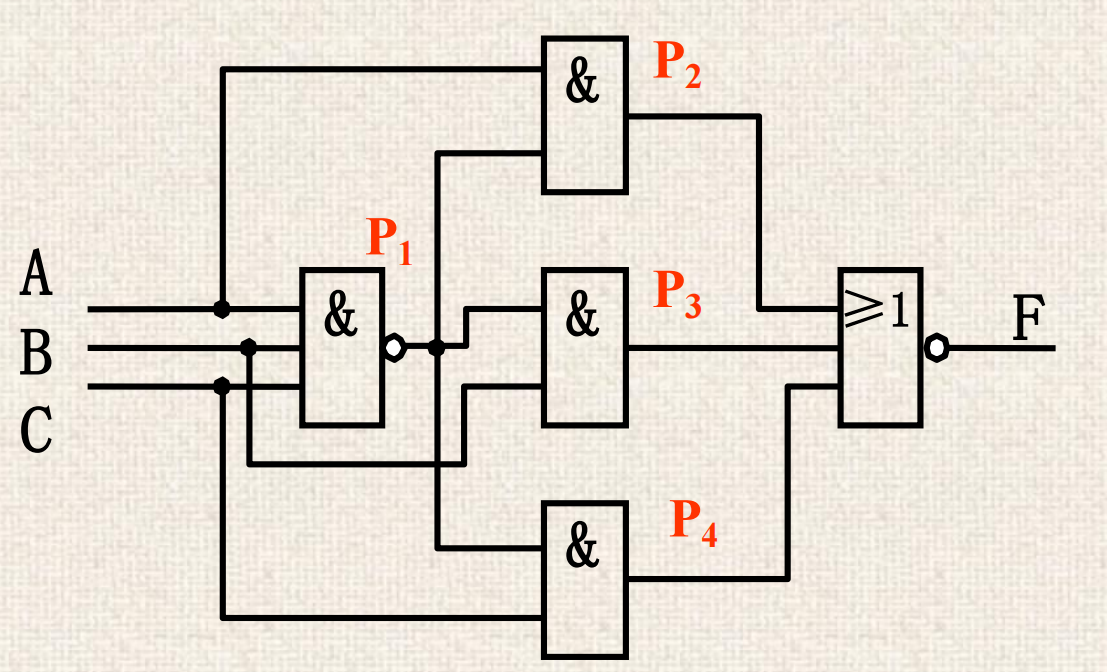
\includegraphics[width=0.5\textwidth]{Figure/组合逻辑电路例题.png}
\end{figure}

采取从后往前分析的方法，把逻辑门输出结果分别标出为$\mathbf{P}_1$、$\mathbf{P}_2$、$\mathbf{P}_3$、$\mathbf{P}_4$。
从后往前分析每一个逻辑门：
$$\mathbf{F}=\overline{\mathbf{P}_2+\mathbf{P}_3+\mathbf{P}_4}$$
$$\mathbf{P}_2=\mathbf{A}\mathbf{P}_1$$
$$\mathbf{P}_3=\mathbf{B}\mathbf{P}_1$$
$$\mathbf{P}_4=\mathbf{C}\mathbf{P}_1$$
$$\mathbf{P}_1=\overline{\mathbf{A}\mathbf{B}\mathbf{C}}$$
$$\mathbf{F}=\overline{(\mathbf{A}+\mathbf{B}+\mathbf{C})\cdot\overline{\mathbf{A}\mathbf{B}\mathbf{C}}}=\mathbf{A}\mathbf{B}\mathbf{C}+\overline{\mathbf{A}}\,\overline{\mathbf{B}}\,\overline{\mathbf{C}}$$

由表达式列出真值表，其中 $\mathbf{P}_1\sim\mathbf{P}_4$ 为图中各逻辑门输出：

\begin{table}[H]
	\centering
	\caption{组合逻辑电路例题真值表}
	\label{tab:真值表:组合逻辑例题}
	\begin{tabular}{ccc|cccc|c}
		\toprule
		$\mathbf{A}$ & $\mathbf{B}$ & $\mathbf{C}$ & $\mathbf{P}_1$ & $\mathbf{P}_2$ & $\mathbf{P}_3$ & $\mathbf{P}_4$ & $\mathbf{F}=\overline{\mathbf{P}_2+\mathbf{P}_3+\mathbf{P}_4}$ \\
		\midrule
		0 & 0 & 0 & 1 & 0 & 0 & 0 & 1 \\
		0 & 0 & 1 & 1 & 0 & 0 & 1 & 0 \\
		0 & 1 & 0 & 1 & 0 & 1 & 0 & 0 \\
		0 & 1 & 1 & 1 & 0 & 1 & 1 & 0 \\
		1 & 0 & 0 & 1 & 1 & 0 & 0 & 0 \\
		1 & 0 & 1 & 1 & 1 & 0 & 1 & 0 \\
		1 & 1 & 0 & 1 & 1 & 1 & 0 & 0 \\
		1 & 1 & 1 & 0 & 0 & 0 & 0 & 1 \\
		\bottomrule
	\end{tabular}
\end{table}

由真值表可知：当且仅当 $\mathbf{A}=\mathbf{B}=\mathbf{C}$ 时 $\mathbf{F}=1$，否则 $\mathbf{F}=0$。即该电路的三个输入取值一致时输出为 1，不一致时输出为 0，实现三变量的“一致”判断（同或）功能。

\subsection{一般设计方法}
一般步骤：
\begin{enumerate}
    \item 由实际问题列出真值表
    \item 由真值表写出逻辑表达式
    \item 化简、变换输出逻辑表达式
    \item 画出逻辑图
\end{enumerate}
如果现在要设计用与非门的一个三变量表决电路,表决规则为少数服从多数，怎么设计？

设由$\mathbf{A} $、$\mathbf{B}$、$\mathbf{C} $表示三个输入变量，$\mathbf{F}$表示表决结果。并设$\mathbf{A} $、$\mathbf{B}$、$\mathbf{C}$为1表示赞成，为0表示反对；$\mathbf{F}$为1表示表决通过，为0 表示不通过。
列出真值表：

\begin{table}[H]
	\centering
	\caption{三变量表决器真值表}
	\label{tab:真值表:表决器}
	\begin{tabular}{ccc|c}
		\toprule
		$\mathbf{A}$ & $\mathbf{B}$ & $\mathbf{C}$ & $\mathbf{F}$ \\
		\midrule
		0 & 0 & 0 & 0 \\
		0 & 0 & 1 & 0 \\
		0 & 1 & 0 & 0 \\
		0 & 1 & 1 & 1 \\
		1 & 0 & 0 & 0 \\
		1 & 0 & 1 & 1 \\
		1 & 1 & 0 & 1 \\
		1 & 1 & 1 & 1 \\
		\bottomrule
	\end{tabular}
\end{table}

由表决规则，三个输入中有两个或两个以上为 1 时表决通过，故 $\mathbf{F}=1$ 对应 $\mathbf{A}\mathbf{B}\mathbf{C}$ 取 $011$、$101$、$110$、$111$ 四种情况。

将 $\mathbf{F}=1$ 的四个最小项 $m_3$、$m_5$、$m_6$、$m_7$ 填入卡诺图并圈组，如图所示：

\begin{figure}[H]
	\centering
	\begin{tikzpicture}
		\matrix (K31) [kmap] {
			|[kmaphead]| $\mathbf{A}\backslash\mathbf{B}\mathbf{C}$ & |[kmaphead]| 00 & |[kmaphead]| 01 & |[kmaphead]| 11 & |[kmaphead]| 10 \\
			|[kmaphead]| 0 & 0 & 0 & 1 & 0 \\
			|[kmaphead]| 1 & 0 & 1 & 1 & 1 \\
		};
		\node[kmapgroup, draw=LiSiThm, fill=LiSiThm, fill opacity=0.06,
			fit=(K31-2-4)(K31-3-4)] {};
		\node[kmapgroup, draw=LiSiWarn, fill=LiSiWarn, fill opacity=0.06,
			fit=(K31-3-3)(K31-3-4)] {};
		\node[kmapgroup, draw=LiSiCor, fill=LiSiCor, fill opacity=0.06,
			fit=(K31-3-5)(K31-3-4)] {};
	\end{tikzpicture}
	\caption{三变量表决电路的卡诺图及圈法}
	\label{fig:卡诺图:表决器}
\end{figure}

图中三个圈分别合并为 $\mathbf{B}\mathbf{C}$、$\mathbf{A}\mathbf{C}$、$\mathbf{A}\mathbf{B}$，故最简与或式为
$$\mathbf{F}=\mathbf{A}\mathbf{B}+\mathbf{B}\mathbf{C}+\mathbf{A}\mathbf{C}=\overline{\overline{\mathbf{A}\mathbf{B}}\cdot\overline{\mathbf{B}\mathbf{C}}\cdot\overline{\mathbf{A}\mathbf{C}}}$$
下一步画出逻辑图，如下图~\ref{fig:逻辑图:表决器}所示：
\begin{figure}[htbp]
    \centering
    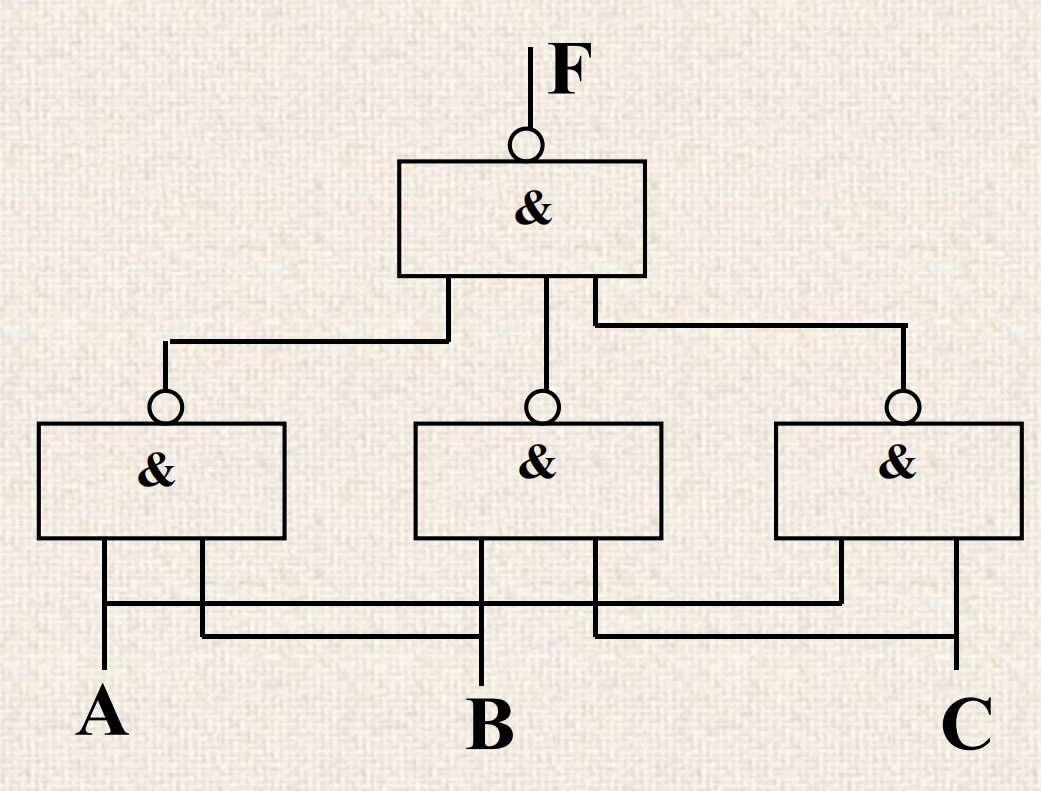
\includegraphics[width=0.5\textwidth]{Figure/组合逻辑电路设计例题.png}
    \caption{三变量表决电路的逻辑图}
    \label{fig:逻辑图:表决器}
\end{figure}

\section{MSI构成的组合逻辑电路}
\subsection{自顶向下的模块化设计方法}
\textcolor{red}{顶}: 指系统功能,即系统总要求,较抽象。

\textcolor{red}{向下}:指根据系统总要求,将系统分解为若干个子系统,再将每个子系统分解为若干个功能模块,直至分成许多各具特定功能的基本模块为止。

如果我现在想设计一个数据检测系统，功能表如下：

\begin{table}[H]
	\centering
	\caption{数据检测系统的功能表}
	\label{tab:功能表:数据检测系统}
	\begin{tabular}{cc|c}
		\toprule
		$\mathbf{S}_1$ & $\mathbf{S}_2$ & 输出功能 \\
		\midrule
		0 & 0 & $\mathbf{A}+\mathbf{B}$ \\
		0 & 1 & $\mathbf{A}-\mathbf{B}$ \\
		1 & 0 & $\mathrm{Min}(\mathbf{A},\mathbf{B})$ \\
		1 & 1 & $\mathrm{Max}(\mathbf{A},\mathbf{B})$ \\
		\bottomrule
	\end{tabular}
\end{table}

其中 $\mathbf{S}_1$、$\mathbf{S}_2$ 为两个子系统，$\mathbf{A}$、$\mathbf{B}$ 为传感器数据输入。

\begin{figure}[H]
	\centering
	\resizebox{\textwidth}{!}{% ============================================================
%  Figure/分层设计树.tex
%  数据检测系统的分层设计树（自顶向下设计方法的分解过程）
%
%  用法（在章节 .tex 中）：
%    \begin{figure}[H]
%        \centering
%        \resizebox{\textwidth}{!}{% ============================================================
%  Figure/分层设计树.tex
%  数据检测系统的分层设计树（自顶向下设计方法的分解过程）
%
%  用法（在章节 .tex 中）：
%    \begin{figure}[H]
%        \centering
%        \resizebox{\textwidth}{!}{% ============================================================
%  Figure/分层设计树.tex
%  数据检测系统的分层设计树（自顶向下设计方法的分解过程）
%
%  用法（在章节 .tex 中）：
%    \begin{figure}[H]
%        \centering
%        \resizebox{\textwidth}{!}{\input{Figure/分层设计树}}
%        \caption{数据检测系统的分层设计树}
%        \label{fig:分层设计树}
%    \end{figure}
%
%  说明：本文件只含一个 tikzpicture，不含 figure 环境，也不排版标题，
%        便于在正文任意位置插入；外面套 \resizebox 可自适应版心宽度。
%        坐标单位为 cm：横向间距按 14pt 基准下各框的实际宽度留出约 0.5cm 空隙
%        （B23/B24 的子节点用横向总线向左扇出，避免整体过宽导致缩放后字太小）。
%        框内字号用 \footnotesize；要整体放大/缩小，只改 box 样式里的 font。
%  依赖：preamble.tex 中的 tikz、xcolor，以及 LiSiThm / LiSiCor / LiSiWarn 配色。
% ============================================================
\providecolor{treeDeep}{RGB}{128,0,176}   % 第三层连线：紫（前两层复用讲义配色）

\begin{tikzpicture}[
	box/.style={draw, thick, align=center, inner sep=3pt, font=\footnotesize},
	leafmark/.style={font=\large},           % 注意：不能叫 mark，TikZ 已占用该键名
	toplink/.style={thick, draw=LiSiThm},    % 顶层 → 子系统：蓝
	midlink/.style={thick, draw=LiSiCor},    % 子系统 → 功能模块：橙
	deeplink/.style={thick, draw=treeDeep}   % 功能模块 → 基本模块：紫
]

	% ------------------------------------------------------------
	%  结点：B 为系统，B1~B3 为子系统，B11~B24 为功能模块，
	%        B231…B242 为基本模块（叶结点）
	% ------------------------------------------------------------
	\node[box] (B)   at (10.56,5.6)  {$\mathbf{B}$: 数据检测系统};

	\node[box] (B1)  at (2.61,3.6)   {$\mathbf{B}_1$: 输入\\传感器数据};
	\node[box] (B2)  at (10.56,3.6)  {$\mathbf{B}_2$\\计算值};
	\node[box] (B3)  at (16.84,3.6)  {$\mathbf{B}_3$\\选择输出};

	\node[box] (B11) at (1.16,1.6)   {$\mathbf{B}_{11}$\\传感器$\mathbf{A}$};
	\node[box] (B12) at (4.05,1.6)   {$\mathbf{B}_{12}$\\传感器$\mathbf{B}$};
	\node[box] (B21) at (6.93,1.6)   {$\mathbf{B}_{21}$\\$\mathbf{A}+\mathbf{B}$};
	\node[box] (B22) at (9.06,1.6)   {$\mathbf{B}_{22}$\\$\mathbf{A}-\mathbf{B}$};
	\node[box] (B23) at (11.44,1.6)  {$\mathbf{B}_{23}$\\$\mathrm{Min}(\mathbf{A},\mathbf{B})$};
	\node[box] (B24) at (14.19,1.6)  {$\mathbf{B}_{24}$\\$\mathrm{Max}(\mathbf{A},\mathbf{B})$};

	\node[box] (B231) at (8.60,-1.6)  {$\mathbf{B}_{231}$\\比较\\$\mathbf{A}$和$\mathbf{B}$};
	\node[box] (B232) at (10.60,-1.6) {$\mathbf{B}_{232}$\\选择\\$\mathrm{Min}$};
	\node[box] (B241) at (12.60,-1.6) {$\mathbf{B}_{241}$\\比较\\$\mathbf{A}$和$\mathbf{B}$};
	\node[box] (B242) at (14.60,-1.6) {$\mathbf{B}_{242}$\\选择\\$\mathrm{Max}$};

	% ------------------------------------------------------------
	%  连线：竖线 + 横向总线，逐层分解
	% ------------------------------------------------------------
	% 顶层 → B1、B2、B3
	\draw[toplink] (B.south) -- (10.56,4.7);
	\draw[toplink] (2.61,4.7) -- (16.84,4.7);
	\draw[toplink] (2.61,4.7)  -- (B1.north);
	\draw[toplink] (10.56,4.7) -- (B2.north);
	\draw[toplink] (16.84,4.7) -- (B3.north);

	% B1 → B11、B12
	\draw[midlink] (B1.south) -- (2.61,2.7);
	\draw[midlink] (1.16,2.7) -- (4.05,2.7);
	\draw[midlink] (1.16,2.7) -- (B11.north);
	\draw[midlink] (4.05,2.7) -- (B12.north);

	% B2 → B21…B24
	\draw[midlink] (B2.south) -- (10.56,2.7);
	\draw[midlink] (6.93,2.7) -- (14.19,2.7);
	\draw[midlink] (6.93,2.7)  -- (B21.north);
	\draw[midlink] (9.06,2.7)  -- (B22.north);
	\draw[midlink] (11.44,2.7) -- (B23.north);
	\draw[midlink] (14.19,2.7) -- (B24.north);

	% B23 → B231、B232（子节点向左扇出，两条横线错开高度以免交叉）
	\draw[deeplink] (B23.south) -- (11.44,-0.15);
	\draw[deeplink] (8.60,-0.15) -- (11.44,-0.15);
	\draw[deeplink] (8.60,-0.15)  -- (B231.north);
	\draw[deeplink] (10.60,-0.15) -- (B232.north);

	% B24 → B241、B242
	\draw[deeplink] (B24.south) -- (14.19,-0.45);
	\draw[deeplink] (12.60,-0.45) -- (14.60,-0.45);
	\draw[deeplink] (12.60,-0.45) -- (B241.north);
	\draw[deeplink] (14.60,-0.45) -- (B242.north);

	% ------------------------------------------------------------
	%  叶结点标记与图例
	% ------------------------------------------------------------
	\foreach \x/\y in {%
		1.16/0.5, 4.05/0.5, 6.93/0.5, 9.06/0.5, 16.84/2.55,%
		8.60/-3.1, 10.60/-3.1, 12.60/-3.1, 14.60/-3.1}{%
		\node[leafmark] at (\x,\y) {$\ast$};%
	}
	\node[anchor=west, font=\footnotesize] at (0.1,-3.1) {$\ast$：叶结点};
	\node[anchor=west, font=\footnotesize\bfseries, text=LiSiWarn] at (12.5,5.6) {顶层};

\end{tikzpicture}
}
%        \caption{数据检测系统的分层设计树}
%        \label{fig:分层设计树}
%    \end{figure}
%
%  说明：本文件只含一个 tikzpicture，不含 figure 环境，也不排版标题，
%        便于在正文任意位置插入；外面套 \resizebox 可自适应版心宽度。
%        坐标单位为 cm：横向间距按 14pt 基准下各框的实际宽度留出约 0.5cm 空隙
%        （B23/B24 的子节点用横向总线向左扇出，避免整体过宽导致缩放后字太小）。
%        框内字号用 \footnotesize；要整体放大/缩小，只改 box 样式里的 font。
%  依赖：preamble.tex 中的 tikz、xcolor，以及 LiSiThm / LiSiCor / LiSiWarn 配色。
% ============================================================
\providecolor{treeDeep}{RGB}{128,0,176}   % 第三层连线：紫（前两层复用讲义配色）

\begin{tikzpicture}[
	box/.style={draw, thick, align=center, inner sep=3pt, font=\footnotesize},
	leafmark/.style={font=\large},           % 注意：不能叫 mark，TikZ 已占用该键名
	toplink/.style={thick, draw=LiSiThm},    % 顶层 → 子系统：蓝
	midlink/.style={thick, draw=LiSiCor},    % 子系统 → 功能模块：橙
	deeplink/.style={thick, draw=treeDeep}   % 功能模块 → 基本模块：紫
]

	% ------------------------------------------------------------
	%  结点：B 为系统，B1~B3 为子系统，B11~B24 为功能模块，
	%        B231…B242 为基本模块（叶结点）
	% ------------------------------------------------------------
	\node[box] (B)   at (10.56,5.6)  {$\mathbf{B}$: 数据检测系统};

	\node[box] (B1)  at (2.61,3.6)   {$\mathbf{B}_1$: 输入\\传感器数据};
	\node[box] (B2)  at (10.56,3.6)  {$\mathbf{B}_2$\\计算值};
	\node[box] (B3)  at (16.84,3.6)  {$\mathbf{B}_3$\\选择输出};

	\node[box] (B11) at (1.16,1.6)   {$\mathbf{B}_{11}$\\传感器$\mathbf{A}$};
	\node[box] (B12) at (4.05,1.6)   {$\mathbf{B}_{12}$\\传感器$\mathbf{B}$};
	\node[box] (B21) at (6.93,1.6)   {$\mathbf{B}_{21}$\\$\mathbf{A}+\mathbf{B}$};
	\node[box] (B22) at (9.06,1.6)   {$\mathbf{B}_{22}$\\$\mathbf{A}-\mathbf{B}$};
	\node[box] (B23) at (11.44,1.6)  {$\mathbf{B}_{23}$\\$\mathrm{Min}(\mathbf{A},\mathbf{B})$};
	\node[box] (B24) at (14.19,1.6)  {$\mathbf{B}_{24}$\\$\mathrm{Max}(\mathbf{A},\mathbf{B})$};

	\node[box] (B231) at (8.60,-1.6)  {$\mathbf{B}_{231}$\\比较\\$\mathbf{A}$和$\mathbf{B}$};
	\node[box] (B232) at (10.60,-1.6) {$\mathbf{B}_{232}$\\选择\\$\mathrm{Min}$};
	\node[box] (B241) at (12.60,-1.6) {$\mathbf{B}_{241}$\\比较\\$\mathbf{A}$和$\mathbf{B}$};
	\node[box] (B242) at (14.60,-1.6) {$\mathbf{B}_{242}$\\选择\\$\mathrm{Max}$};

	% ------------------------------------------------------------
	%  连线：竖线 + 横向总线，逐层分解
	% ------------------------------------------------------------
	% 顶层 → B1、B2、B3
	\draw[toplink] (B.south) -- (10.56,4.7);
	\draw[toplink] (2.61,4.7) -- (16.84,4.7);
	\draw[toplink] (2.61,4.7)  -- (B1.north);
	\draw[toplink] (10.56,4.7) -- (B2.north);
	\draw[toplink] (16.84,4.7) -- (B3.north);

	% B1 → B11、B12
	\draw[midlink] (B1.south) -- (2.61,2.7);
	\draw[midlink] (1.16,2.7) -- (4.05,2.7);
	\draw[midlink] (1.16,2.7) -- (B11.north);
	\draw[midlink] (4.05,2.7) -- (B12.north);

	% B2 → B21…B24
	\draw[midlink] (B2.south) -- (10.56,2.7);
	\draw[midlink] (6.93,2.7) -- (14.19,2.7);
	\draw[midlink] (6.93,2.7)  -- (B21.north);
	\draw[midlink] (9.06,2.7)  -- (B22.north);
	\draw[midlink] (11.44,2.7) -- (B23.north);
	\draw[midlink] (14.19,2.7) -- (B24.north);

	% B23 → B231、B232（子节点向左扇出，两条横线错开高度以免交叉）
	\draw[deeplink] (B23.south) -- (11.44,-0.15);
	\draw[deeplink] (8.60,-0.15) -- (11.44,-0.15);
	\draw[deeplink] (8.60,-0.15)  -- (B231.north);
	\draw[deeplink] (10.60,-0.15) -- (B232.north);

	% B24 → B241、B242
	\draw[deeplink] (B24.south) -- (14.19,-0.45);
	\draw[deeplink] (12.60,-0.45) -- (14.60,-0.45);
	\draw[deeplink] (12.60,-0.45) -- (B241.north);
	\draw[deeplink] (14.60,-0.45) -- (B242.north);

	% ------------------------------------------------------------
	%  叶结点标记与图例
	% ------------------------------------------------------------
	\foreach \x/\y in {%
		1.16/0.5, 4.05/0.5, 6.93/0.5, 9.06/0.5, 16.84/2.55,%
		8.60/-3.1, 10.60/-3.1, 12.60/-3.1, 14.60/-3.1}{%
		\node[leafmark] at (\x,\y) {$\ast$};%
	}
	\node[anchor=west, font=\footnotesize] at (0.1,-3.1) {$\ast$：叶结点};
	\node[anchor=west, font=\footnotesize\bfseries, text=LiSiWarn] at (12.5,5.6) {顶层};

\end{tikzpicture}
}
%        \caption{数据检测系统的分层设计树}
%        \label{fig:分层设计树}
%    \end{figure}
%
%  说明：本文件只含一个 tikzpicture，不含 figure 环境，也不排版标题，
%        便于在正文任意位置插入；外面套 \resizebox 可自适应版心宽度。
%        坐标单位为 cm：横向间距按 14pt 基准下各框的实际宽度留出约 0.5cm 空隙
%        （B23/B24 的子节点用横向总线向左扇出，避免整体过宽导致缩放后字太小）。
%        框内字号用 \footnotesize；要整体放大/缩小，只改 box 样式里的 font。
%  依赖：preamble.tex 中的 tikz、xcolor，以及 LiSiThm / LiSiCor / LiSiWarn 配色。
% ============================================================
\providecolor{treeDeep}{RGB}{128,0,176}   % 第三层连线：紫（前两层复用讲义配色）

\begin{tikzpicture}[
	box/.style={draw, thick, align=center, inner sep=3pt, font=\footnotesize},
	leafmark/.style={font=\large},           % 注意：不能叫 mark，TikZ 已占用该键名
	toplink/.style={thick, draw=LiSiThm},    % 顶层 → 子系统：蓝
	midlink/.style={thick, draw=LiSiCor},    % 子系统 → 功能模块：橙
	deeplink/.style={thick, draw=treeDeep}   % 功能模块 → 基本模块：紫
]

	% ------------------------------------------------------------
	%  结点：B 为系统，B1~B3 为子系统，B11~B24 为功能模块，
	%        B231…B242 为基本模块（叶结点）
	% ------------------------------------------------------------
	\node[box] (B)   at (10.56,5.6)  {$\mathbf{B}$: 数据检测系统};

	\node[box] (B1)  at (2.61,3.6)   {$\mathbf{B}_1$: 输入\\传感器数据};
	\node[box] (B2)  at (10.56,3.6)  {$\mathbf{B}_2$\\计算值};
	\node[box] (B3)  at (16.84,3.6)  {$\mathbf{B}_3$\\选择输出};

	\node[box] (B11) at (1.16,1.6)   {$\mathbf{B}_{11}$\\传感器$\mathbf{A}$};
	\node[box] (B12) at (4.05,1.6)   {$\mathbf{B}_{12}$\\传感器$\mathbf{B}$};
	\node[box] (B21) at (6.93,1.6)   {$\mathbf{B}_{21}$\\$\mathbf{A}+\mathbf{B}$};
	\node[box] (B22) at (9.06,1.6)   {$\mathbf{B}_{22}$\\$\mathbf{A}-\mathbf{B}$};
	\node[box] (B23) at (11.44,1.6)  {$\mathbf{B}_{23}$\\$\mathrm{Min}(\mathbf{A},\mathbf{B})$};
	\node[box] (B24) at (14.19,1.6)  {$\mathbf{B}_{24}$\\$\mathrm{Max}(\mathbf{A},\mathbf{B})$};

	\node[box] (B231) at (8.60,-1.6)  {$\mathbf{B}_{231}$\\比较\\$\mathbf{A}$和$\mathbf{B}$};
	\node[box] (B232) at (10.60,-1.6) {$\mathbf{B}_{232}$\\选择\\$\mathrm{Min}$};
	\node[box] (B241) at (12.60,-1.6) {$\mathbf{B}_{241}$\\比较\\$\mathbf{A}$和$\mathbf{B}$};
	\node[box] (B242) at (14.60,-1.6) {$\mathbf{B}_{242}$\\选择\\$\mathrm{Max}$};

	% ------------------------------------------------------------
	%  连线：竖线 + 横向总线，逐层分解
	% ------------------------------------------------------------
	% 顶层 → B1、B2、B3
	\draw[toplink] (B.south) -- (10.56,4.7);
	\draw[toplink] (2.61,4.7) -- (16.84,4.7);
	\draw[toplink] (2.61,4.7)  -- (B1.north);
	\draw[toplink] (10.56,4.7) -- (B2.north);
	\draw[toplink] (16.84,4.7) -- (B3.north);

	% B1 → B11、B12
	\draw[midlink] (B1.south) -- (2.61,2.7);
	\draw[midlink] (1.16,2.7) -- (4.05,2.7);
	\draw[midlink] (1.16,2.7) -- (B11.north);
	\draw[midlink] (4.05,2.7) -- (B12.north);

	% B2 → B21…B24
	\draw[midlink] (B2.south) -- (10.56,2.7);
	\draw[midlink] (6.93,2.7) -- (14.19,2.7);
	\draw[midlink] (6.93,2.7)  -- (B21.north);
	\draw[midlink] (9.06,2.7)  -- (B22.north);
	\draw[midlink] (11.44,2.7) -- (B23.north);
	\draw[midlink] (14.19,2.7) -- (B24.north);

	% B23 → B231、B232（子节点向左扇出，两条横线错开高度以免交叉）
	\draw[deeplink] (B23.south) -- (11.44,-0.15);
	\draw[deeplink] (8.60,-0.15) -- (11.44,-0.15);
	\draw[deeplink] (8.60,-0.15)  -- (B231.north);
	\draw[deeplink] (10.60,-0.15) -- (B232.north);

	% B24 → B241、B242
	\draw[deeplink] (B24.south) -- (14.19,-0.45);
	\draw[deeplink] (12.60,-0.45) -- (14.60,-0.45);
	\draw[deeplink] (12.60,-0.45) -- (B241.north);
	\draw[deeplink] (14.60,-0.45) -- (B242.north);

	% ------------------------------------------------------------
	%  叶结点标记与图例
	% ------------------------------------------------------------
	\foreach \x/\y in {%
		1.16/0.5, 4.05/0.5, 6.93/0.5, 9.06/0.5, 16.84/2.55,%
		8.60/-3.1, 10.60/-3.1, 12.60/-3.1, 14.60/-3.1}{%
		\node[leafmark] at (\x,\y) {$\ast$};%
	}
	\node[anchor=west, font=\footnotesize] at (0.1,-3.1) {$\ast$：叶结点};
	\node[anchor=west, font=\footnotesize\bfseries, text=LiSiWarn] at (12.5,5.6) {顶层};

\end{tikzpicture}
}
	\caption{数据检测系统的分层设计树}
	\label{fig:分层设计树}
\end{figure}

各模块之间的信号连接关系如图~\ref{fig:分层方框图}所示：

\begin{figure}[H]
	\centering
	\resizebox{\textwidth}{!}{% ============================================================
%  Figure/分层方框图.tex
%  数据检测系统的分层方框图（各模块之间的信号互联关系）
%
%  用法（在章节 .tex 中）：
%    \begin{figure}[H]
%        \centering
%        \resizebox{\textwidth}{!}{% ============================================================
%  Figure/分层方框图.tex
%  数据检测系统的分层方框图（各模块之间的信号互联关系）
%
%  用法（在章节 .tex 中）：
%    \begin{figure}[H]
%        \centering
%        \resizebox{\textwidth}{!}{% ============================================================
%  Figure/分层方框图.tex
%  数据检测系统的分层方框图（各模块之间的信号互联关系）
%
%  用法（在章节 .tex 中）：
%    \begin{figure}[H]
%        \centering
%        \resizebox{\textwidth}{!}{\input{Figure/分层方框图}}
%        \caption{数据检测系统的分层方框图}
%        \label{fig:分层方框图}
%    \end{figure}
%
%  说明：本文件只含一个 tikzpicture，不含 figure 环境，也不排版标题。
%        坐标单位 cm，整体按课件原图比例布置（约 16cm × 10cm），
%        外层 \resizebox 保证缩放后正好占满版心。
%        自定义样式统一带 d 前缀，避免与 TikZ 内置键重名（如内置的 mark / port）。
%  依赖：preamble.tex 的 tikz、xcolor 与 LiSiThm / LiSiWarn 配色；本文件自带 shapes.symbols。
% ============================================================
\usetikzlibrary{shapes.symbols}   % 输入/输出端口用的 signal（五边形）形状

\begin{tikzpicture}[
	dblk/.style={draw, thick, align=center, font=\footnotesize, inner sep=2pt},
	dwire/.style={thick, -{Stealth[length=1.6mm, width=1.2mm]}},
	dbus/.style={thick},
	dgrp/.style={thick, dotted},
	dbgrp/.style={thick, dashed},
	din/.style={signal, draw, thick, signal to=east, font=\footnotesize,
	           minimum height=0.55cm, minimum width=0.90cm, inner sep=1pt},
	dout/.style={signal, draw, thick, signal to=south, font=\footnotesize,
	             minimum height=0.60cm, minimum width=0.55cm, inner sep=0pt},
	dred/.style={font=\footnotesize\bfseries, text=LiSiWarn},
	dblue/.style={font=\footnotesize, text=LiSiThm},
	dlab/.style={font=\footnotesize}
]

	% ------------------------------------------------------------
	%  输入 / 输出端口
	% ------------------------------------------------------------
	\node[din] (A)  at (1.00,8.76) {$\mathbf{A}$};
	\node[din] (B)  at (1.00,7.36) {$\mathbf{B}$};
	\node[din] (S1) at (1.05,2.21) {$\mathbf{S}_1$};
	\node[din] (S2) at (1.05,1.61) {$\mathbf{S}_2$};
	\node[dout] (OUT) at (7.85,0.00) {};

	% ------------------------------------------------------------
	%  各级模块方框
	% ------------------------------------------------------------
	\node[dblk, minimum width=1.60cm, minimum height=1.05cm] (B11) at (2.65,8.76)  {$\mathbf{B}_{11}$\\转换$\mathbf{A}$};
	\node[dblk, minimum width=1.60cm, minimum height=1.05cm] (B12) at (2.65,7.36)  {$\mathbf{B}_{12}$\\转换$\mathbf{B}$};
	\node[dblk, minimum width=1.55cm, minimum height=1.55cm] (B21) at (4.72,5.71)  {$\mathbf{B}_{21}$\\二进制\\加法};
	\node[dblk, minimum width=1.55cm, minimum height=1.55cm] (B22) at (6.78,5.71)  {$\mathbf{B}_{22}$\\二进制\\减法};
	\node[dblk, minimum width=1.50cm, minimum height=1.10cm] (B231) at (8.85,4.21)  {$\mathbf{B}_{231}$\\比较};
	\node[dblk, minimum width=1.50cm, minimum height=1.10cm] (B232) at (10.85,4.21) {$\mathbf{B}_{232}$\\选择};
	\node[dblk, minimum width=1.50cm, minimum height=1.10cm] (B241) at (13.10,4.21) {$\mathbf{B}_{241}$\\比较};
	\node[dblk, minimum width=1.50cm, minimum height=1.10cm] (B242) at (15.00,4.21) {$\mathbf{B}_{242}$\\选择};
	\node[dblk, minimum width=3.90cm, minimum height=1.25cm] (B3)   at (7.85,1.79)  {$\mathbf{B}_3$\\输出选择};

	% ------------------------------------------------------------
	%  分组虚线/点线框
	% ------------------------------------------------------------
	\draw[dgrp]  (1.75,6.66) rectangle (3.55,9.46);      % B1：输入
	\draw[dbgrp] (3.85,3.10) rectangle (16.00,9.50);     % B2：计算
	\draw[dgrp]  (7.95,3.31) rectangle (11.80,5.81);     % B23：min
	\draw[dgrp]  (12.15,3.31) rectangle (15.90,5.81);    % B24：max

	% ------------------------------------------------------------
	%  连线：A、B 两条总线分别送到六个功能模块
	%  （A 总线在上、B 总线在下；A 的下引线穿过 B 总线处为不连接的交叉）
	% ------------------------------------------------------------
	\draw[dbus] (B11.east) -- (14.50,8.76);   % A 总线
	\draw[dbus] (B12.east) -- (15.40,7.36);   % B 总线

	% A 总线 → 各模块左侧输入
	\draw[dwire] (4.30,8.76)  -- (4.30,6.485);    % B21
	\draw[dwire] (6.35,8.76)  -- (6.35,6.485);    % B22
	\draw[dwire] (8.35,8.76)  -- (8.35,4.76);     % B231
	\draw[dwire] (10.35,8.76) -- (10.35,4.76);    % B232
	\draw[dwire] (12.90,8.76) -- (12.90,4.76);    % B241
	\draw[dwire] (14.50,8.76) -- (14.50,4.76);    % B242

	% B 总线 → 各模块右侧输入
	\draw[dwire] (5.15,7.36)  -- (5.15,6.485);    % B21
	\draw[dwire] (7.20,7.36)  -- (7.20,6.485);    % B22
	\draw[dwire] (9.20,7.36)  -- (9.20,4.76);     % B231
	\draw[dwire] (11.05,7.36) -- (11.05,4.76);    % B232
	\draw[dwire] (13.55,7.36) -- (13.55,4.76);    % B241
	\draw[dwire] (15.40,7.36) -- (15.40,4.76);    % B242

	% 传感器 → B11、B12
	\draw[dwire] (A.east) -- (B11.west);
	\draw[dwire] (B.east) -- (B12.west);

	% 比较 → 选择
	\draw[dwire] (B231.east) -- (B232.west);
	\draw[dwire] (B241.east) -- (B242.west);

	% 加法、减法 → 输出选择
	\draw[dwire] (4.72,4.935) -- (4.72,2.95) -- (6.55,2.95) -- (6.55,2.415);
	\draw[dwire] (6.78,4.935) -- (6.78,2.80) -- (7.15,2.80) -- (7.15,2.415);

	% min、max 的选择结果 → 输出选择（两条横线错开高度，避免重叠）
	\draw[dwire] (10.85,3.66) -- (10.85,3.22) -- (8.45,3.22) -- (8.45,2.415);
	\draw[dwire] (15.00,3.66) -- (15.00,2.88) -- (9.35,2.88) -- (9.35,2.415);

	% 功能选择 S1、S2 → 输出选择
	\draw[dwire] (S1.east) -- (5.90,2.21);
	\draw[dwire] (S2.east) -- (5.90,1.61);

	% 输出选择 → 输出端口
	\draw[dwire] (7.85,1.165) -- (7.85,0.35);

	% ------------------------------------------------------------
	%  文字标注（红字为课件上的分组名，蓝字为被测量的物理量）
	% ------------------------------------------------------------
	\node[dred]  at (2.65,6.30)   {$\mathbf{B}_1$: 输入};
	\node[dred]  at (11.60,9.20)  {$\mathbf{B}_2$: 计算};
	\node[dred]  at (1.45,0.95)   {功能选择};
	\node[dred, anchor=west] at (8.35,0.05) {输出};
	\node[dblue, rotate=90] at (0.40,6.65) {传感器};

	\node[dlab] at (9.78,5.45)  {\textbf{min}};
	\node[dlab] at (11.45,5.45) {$\mathbf{B}_{23}$};
	\node[dlab] at (12.42,5.45) {$\mathbf{B}_{24}$};
	\node[dlab] at (13.98,5.45) {\textbf{max}};

\end{tikzpicture}
}
%        \caption{数据检测系统的分层方框图}
%        \label{fig:分层方框图}
%    \end{figure}
%
%  说明：本文件只含一个 tikzpicture，不含 figure 环境，也不排版标题。
%        坐标单位 cm，整体按课件原图比例布置（约 16cm × 10cm），
%        外层 \resizebox 保证缩放后正好占满版心。
%        自定义样式统一带 d 前缀，避免与 TikZ 内置键重名（如内置的 mark / port）。
%  依赖：preamble.tex 的 tikz、xcolor 与 LiSiThm / LiSiWarn 配色；本文件自带 shapes.symbols。
% ============================================================
\usetikzlibrary{shapes.symbols}   % 输入/输出端口用的 signal（五边形）形状

\begin{tikzpicture}[
	dblk/.style={draw, thick, align=center, font=\footnotesize, inner sep=2pt},
	dwire/.style={thick, -{Stealth[length=1.6mm, width=1.2mm]}},
	dbus/.style={thick},
	dgrp/.style={thick, dotted},
	dbgrp/.style={thick, dashed},
	din/.style={signal, draw, thick, signal to=east, font=\footnotesize,
	           minimum height=0.55cm, minimum width=0.90cm, inner sep=1pt},
	dout/.style={signal, draw, thick, signal to=south, font=\footnotesize,
	             minimum height=0.60cm, minimum width=0.55cm, inner sep=0pt},
	dred/.style={font=\footnotesize\bfseries, text=LiSiWarn},
	dblue/.style={font=\footnotesize, text=LiSiThm},
	dlab/.style={font=\footnotesize}
]

	% ------------------------------------------------------------
	%  输入 / 输出端口
	% ------------------------------------------------------------
	\node[din] (A)  at (1.00,8.76) {$\mathbf{A}$};
	\node[din] (B)  at (1.00,7.36) {$\mathbf{B}$};
	\node[din] (S1) at (1.05,2.21) {$\mathbf{S}_1$};
	\node[din] (S2) at (1.05,1.61) {$\mathbf{S}_2$};
	\node[dout] (OUT) at (7.85,0.00) {};

	% ------------------------------------------------------------
	%  各级模块方框
	% ------------------------------------------------------------
	\node[dblk, minimum width=1.60cm, minimum height=1.05cm] (B11) at (2.65,8.76)  {$\mathbf{B}_{11}$\\转换$\mathbf{A}$};
	\node[dblk, minimum width=1.60cm, minimum height=1.05cm] (B12) at (2.65,7.36)  {$\mathbf{B}_{12}$\\转换$\mathbf{B}$};
	\node[dblk, minimum width=1.55cm, minimum height=1.55cm] (B21) at (4.72,5.71)  {$\mathbf{B}_{21}$\\二进制\\加法};
	\node[dblk, minimum width=1.55cm, minimum height=1.55cm] (B22) at (6.78,5.71)  {$\mathbf{B}_{22}$\\二进制\\减法};
	\node[dblk, minimum width=1.50cm, minimum height=1.10cm] (B231) at (8.85,4.21)  {$\mathbf{B}_{231}$\\比较};
	\node[dblk, minimum width=1.50cm, minimum height=1.10cm] (B232) at (10.85,4.21) {$\mathbf{B}_{232}$\\选择};
	\node[dblk, minimum width=1.50cm, minimum height=1.10cm] (B241) at (13.10,4.21) {$\mathbf{B}_{241}$\\比较};
	\node[dblk, minimum width=1.50cm, minimum height=1.10cm] (B242) at (15.00,4.21) {$\mathbf{B}_{242}$\\选择};
	\node[dblk, minimum width=3.90cm, minimum height=1.25cm] (B3)   at (7.85,1.79)  {$\mathbf{B}_3$\\输出选择};

	% ------------------------------------------------------------
	%  分组虚线/点线框
	% ------------------------------------------------------------
	\draw[dgrp]  (1.75,6.66) rectangle (3.55,9.46);      % B1：输入
	\draw[dbgrp] (3.85,3.10) rectangle (16.00,9.50);     % B2：计算
	\draw[dgrp]  (7.95,3.31) rectangle (11.80,5.81);     % B23：min
	\draw[dgrp]  (12.15,3.31) rectangle (15.90,5.81);    % B24：max

	% ------------------------------------------------------------
	%  连线：A、B 两条总线分别送到六个功能模块
	%  （A 总线在上、B 总线在下；A 的下引线穿过 B 总线处为不连接的交叉）
	% ------------------------------------------------------------
	\draw[dbus] (B11.east) -- (14.50,8.76);   % A 总线
	\draw[dbus] (B12.east) -- (15.40,7.36);   % B 总线

	% A 总线 → 各模块左侧输入
	\draw[dwire] (4.30,8.76)  -- (4.30,6.485);    % B21
	\draw[dwire] (6.35,8.76)  -- (6.35,6.485);    % B22
	\draw[dwire] (8.35,8.76)  -- (8.35,4.76);     % B231
	\draw[dwire] (10.35,8.76) -- (10.35,4.76);    % B232
	\draw[dwire] (12.90,8.76) -- (12.90,4.76);    % B241
	\draw[dwire] (14.50,8.76) -- (14.50,4.76);    % B242

	% B 总线 → 各模块右侧输入
	\draw[dwire] (5.15,7.36)  -- (5.15,6.485);    % B21
	\draw[dwire] (7.20,7.36)  -- (7.20,6.485);    % B22
	\draw[dwire] (9.20,7.36)  -- (9.20,4.76);     % B231
	\draw[dwire] (11.05,7.36) -- (11.05,4.76);    % B232
	\draw[dwire] (13.55,7.36) -- (13.55,4.76);    % B241
	\draw[dwire] (15.40,7.36) -- (15.40,4.76);    % B242

	% 传感器 → B11、B12
	\draw[dwire] (A.east) -- (B11.west);
	\draw[dwire] (B.east) -- (B12.west);

	% 比较 → 选择
	\draw[dwire] (B231.east) -- (B232.west);
	\draw[dwire] (B241.east) -- (B242.west);

	% 加法、减法 → 输出选择
	\draw[dwire] (4.72,4.935) -- (4.72,2.95) -- (6.55,2.95) -- (6.55,2.415);
	\draw[dwire] (6.78,4.935) -- (6.78,2.80) -- (7.15,2.80) -- (7.15,2.415);

	% min、max 的选择结果 → 输出选择（两条横线错开高度，避免重叠）
	\draw[dwire] (10.85,3.66) -- (10.85,3.22) -- (8.45,3.22) -- (8.45,2.415);
	\draw[dwire] (15.00,3.66) -- (15.00,2.88) -- (9.35,2.88) -- (9.35,2.415);

	% 功能选择 S1、S2 → 输出选择
	\draw[dwire] (S1.east) -- (5.90,2.21);
	\draw[dwire] (S2.east) -- (5.90,1.61);

	% 输出选择 → 输出端口
	\draw[dwire] (7.85,1.165) -- (7.85,0.35);

	% ------------------------------------------------------------
	%  文字标注（红字为课件上的分组名，蓝字为被测量的物理量）
	% ------------------------------------------------------------
	\node[dred]  at (2.65,6.30)   {$\mathbf{B}_1$: 输入};
	\node[dred]  at (11.60,9.20)  {$\mathbf{B}_2$: 计算};
	\node[dred]  at (1.45,0.95)   {功能选择};
	\node[dred, anchor=west] at (8.35,0.05) {输出};
	\node[dblue, rotate=90] at (0.40,6.65) {传感器};

	\node[dlab] at (9.78,5.45)  {\textbf{min}};
	\node[dlab] at (11.45,5.45) {$\mathbf{B}_{23}$};
	\node[dlab] at (12.42,5.45) {$\mathbf{B}_{24}$};
	\node[dlab] at (13.98,5.45) {\textbf{max}};

\end{tikzpicture}
}
%        \caption{数据检测系统的分层方框图}
%        \label{fig:分层方框图}
%    \end{figure}
%
%  说明：本文件只含一个 tikzpicture，不含 figure 环境，也不排版标题。
%        坐标单位 cm，整体按课件原图比例布置（约 16cm × 10cm），
%        外层 \resizebox 保证缩放后正好占满版心。
%        自定义样式统一带 d 前缀，避免与 TikZ 内置键重名（如内置的 mark / port）。
%  依赖：preamble.tex 的 tikz、xcolor 与 LiSiThm / LiSiWarn 配色；本文件自带 shapes.symbols。
% ============================================================
\usetikzlibrary{shapes.symbols}   % 输入/输出端口用的 signal（五边形）形状

\begin{tikzpicture}[
	dblk/.style={draw, thick, align=center, font=\footnotesize, inner sep=2pt},
	dwire/.style={thick, -{Stealth[length=1.6mm, width=1.2mm]}},
	dbus/.style={thick},
	dgrp/.style={thick, dotted},
	dbgrp/.style={thick, dashed},
	din/.style={signal, draw, thick, signal to=east, font=\footnotesize,
	           minimum height=0.55cm, minimum width=0.90cm, inner sep=1pt},
	dout/.style={signal, draw, thick, signal to=south, font=\footnotesize,
	             minimum height=0.60cm, minimum width=0.55cm, inner sep=0pt},
	dred/.style={font=\footnotesize\bfseries, text=LiSiWarn},
	dblue/.style={font=\footnotesize, text=LiSiThm},
	dlab/.style={font=\footnotesize}
]

	% ------------------------------------------------------------
	%  输入 / 输出端口
	% ------------------------------------------------------------
	\node[din] (A)  at (1.00,8.76) {$\mathbf{A}$};
	\node[din] (B)  at (1.00,7.36) {$\mathbf{B}$};
	\node[din] (S1) at (1.05,2.21) {$\mathbf{S}_1$};
	\node[din] (S2) at (1.05,1.61) {$\mathbf{S}_2$};
	\node[dout] (OUT) at (7.85,0.00) {};

	% ------------------------------------------------------------
	%  各级模块方框
	% ------------------------------------------------------------
	\node[dblk, minimum width=1.60cm, minimum height=1.05cm] (B11) at (2.65,8.76)  {$\mathbf{B}_{11}$\\转换$\mathbf{A}$};
	\node[dblk, minimum width=1.60cm, minimum height=1.05cm] (B12) at (2.65,7.36)  {$\mathbf{B}_{12}$\\转换$\mathbf{B}$};
	\node[dblk, minimum width=1.55cm, minimum height=1.55cm] (B21) at (4.72,5.71)  {$\mathbf{B}_{21}$\\二进制\\加法};
	\node[dblk, minimum width=1.55cm, minimum height=1.55cm] (B22) at (6.78,5.71)  {$\mathbf{B}_{22}$\\二进制\\减法};
	\node[dblk, minimum width=1.50cm, minimum height=1.10cm] (B231) at (8.85,4.21)  {$\mathbf{B}_{231}$\\比较};
	\node[dblk, minimum width=1.50cm, minimum height=1.10cm] (B232) at (10.85,4.21) {$\mathbf{B}_{232}$\\选择};
	\node[dblk, minimum width=1.50cm, minimum height=1.10cm] (B241) at (13.10,4.21) {$\mathbf{B}_{241}$\\比较};
	\node[dblk, minimum width=1.50cm, minimum height=1.10cm] (B242) at (15.00,4.21) {$\mathbf{B}_{242}$\\选择};
	\node[dblk, minimum width=3.90cm, minimum height=1.25cm] (B3)   at (7.85,1.79)  {$\mathbf{B}_3$\\输出选择};

	% ------------------------------------------------------------
	%  分组虚线/点线框
	% ------------------------------------------------------------
	\draw[dgrp]  (1.75,6.66) rectangle (3.55,9.46);      % B1：输入
	\draw[dbgrp] (3.85,3.10) rectangle (16.00,9.50);     % B2：计算
	\draw[dgrp]  (7.95,3.31) rectangle (11.80,5.81);     % B23：min
	\draw[dgrp]  (12.15,3.31) rectangle (15.90,5.81);    % B24：max

	% ------------------------------------------------------------
	%  连线：A、B 两条总线分别送到六个功能模块
	%  （A 总线在上、B 总线在下；A 的下引线穿过 B 总线处为不连接的交叉）
	% ------------------------------------------------------------
	\draw[dbus] (B11.east) -- (14.50,8.76);   % A 总线
	\draw[dbus] (B12.east) -- (15.40,7.36);   % B 总线

	% A 总线 → 各模块左侧输入
	\draw[dwire] (4.30,8.76)  -- (4.30,6.485);    % B21
	\draw[dwire] (6.35,8.76)  -- (6.35,6.485);    % B22
	\draw[dwire] (8.35,8.76)  -- (8.35,4.76);     % B231
	\draw[dwire] (10.35,8.76) -- (10.35,4.76);    % B232
	\draw[dwire] (12.90,8.76) -- (12.90,4.76);    % B241
	\draw[dwire] (14.50,8.76) -- (14.50,4.76);    % B242

	% B 总线 → 各模块右侧输入
	\draw[dwire] (5.15,7.36)  -- (5.15,6.485);    % B21
	\draw[dwire] (7.20,7.36)  -- (7.20,6.485);    % B22
	\draw[dwire] (9.20,7.36)  -- (9.20,4.76);     % B231
	\draw[dwire] (11.05,7.36) -- (11.05,4.76);    % B232
	\draw[dwire] (13.55,7.36) -- (13.55,4.76);    % B241
	\draw[dwire] (15.40,7.36) -- (15.40,4.76);    % B242

	% 传感器 → B11、B12
	\draw[dwire] (A.east) -- (B11.west);
	\draw[dwire] (B.east) -- (B12.west);

	% 比较 → 选择
	\draw[dwire] (B231.east) -- (B232.west);
	\draw[dwire] (B241.east) -- (B242.west);

	% 加法、减法 → 输出选择
	\draw[dwire] (4.72,4.935) -- (4.72,2.95) -- (6.55,2.95) -- (6.55,2.415);
	\draw[dwire] (6.78,4.935) -- (6.78,2.80) -- (7.15,2.80) -- (7.15,2.415);

	% min、max 的选择结果 → 输出选择（两条横线错开高度，避免重叠）
	\draw[dwire] (10.85,3.66) -- (10.85,3.22) -- (8.45,3.22) -- (8.45,2.415);
	\draw[dwire] (15.00,3.66) -- (15.00,2.88) -- (9.35,2.88) -- (9.35,2.415);

	% 功能选择 S1、S2 → 输出选择
	\draw[dwire] (S1.east) -- (5.90,2.21);
	\draw[dwire] (S2.east) -- (5.90,1.61);

	% 输出选择 → 输出端口
	\draw[dwire] (7.85,1.165) -- (7.85,0.35);

	% ------------------------------------------------------------
	%  文字标注（红字为课件上的分组名，蓝字为被测量的物理量）
	% ------------------------------------------------------------
	\node[dred]  at (2.65,6.30)   {$\mathbf{B}_1$: 输入};
	\node[dred]  at (11.60,9.20)  {$\mathbf{B}_2$: 计算};
	\node[dred]  at (1.45,0.95)   {功能选择};
	\node[dred, anchor=west] at (8.35,0.05) {输出};
	\node[dblue, rotate=90] at (0.40,6.65) {传感器};

	\node[dlab] at (9.78,5.45)  {\textbf{min}};
	\node[dlab] at (11.45,5.45) {$\mathbf{B}_{23}$};
	\node[dlab] at (12.42,5.45) {$\mathbf{B}_{24}$};
	\node[dlab] at (13.98,5.45) {\textbf{max}};

\end{tikzpicture}
}
	\caption{数据检测系统的分层方框图}
	\label{fig:分层方框图}
\end{figure}

这样，我们就完成了一个系统的模块化设计。

\subsection{编码器}
编码器能够将信息(如数和字符等)转换成符合一定规则的二进制代码。

\subsubsection{二进制编码器}
用$n$位二进制代码对$N=2^n$个特定信息进行编码的逻辑电路.

下面说明一下二进制编码器的设计方法。

假设咱们现在需要设计一个具有互相排斥输入条件的编码器。

输入为$\mathbf{X_0}$、$\mathbf{X_1}$、$\mathbf{X_2}$、$\mathbf{X_3}$，输出为$\mathbf{A_0}$、$\mathbf{A_1}$。
具有如下对应关系：
\begin{table}[H]
	\centering
	\caption{二进制编码器的输入输出对应关系}
	\label{tab:二进制编码器输入输出对应关系}
	\begin{tabular}{c|cc}
		\toprule
		输入 &$\mathbf{A_1}$  & $\mathbf{A_0}$ \\
		\midrule
		$\mathbf{X_0}$ & 0 & 0 \\
		$\mathbf{X_1}$ & 0 & 1 \\
		$\mathbf{X_2}$ & 1 & 0 \\
		$\mathbf{X_3}$ & 1 & 1 \\
		\bottomrule
	\end{tabular}
\end{table}
